%
%  --- USU thesis and dissertation template ---
%
% Time-stamp: "[thesis.tex] last modified by Scott Budge (scott) on 2016-09-12 (Monday, 12 September 2016) at 16:47:12 on goga.ece.usu.edu"
%
%  Modified to use the new usuthesis.cls by Allan McInnes
%
%  Specify department ('ee' or 'ce' or 'mae') and document type ('msthesis',
%  'msreport', or 'dissertation') in the documentclass options. 
%
%  Including the 'proposal' option will generate a proposal for a thesis
%  or dissertation, rather than a final document (this mostly just 
%  alters the cover page).
%
%  See the opening comments of usuthesis.cls for more information on 
%  available options
%
%  To create finished document run:
%    latex thesis.tex
%    bibtex thesis (or sample-chapter1, etc., if using multiple-paper format)
%    latex thesis.tex
%    latex thesis.tex
%
%  Info: $Id: thesis.tex 967 2016-07-28 15:33:29Z scott $   USU
%  Revision: $Rev: 967 $
% $LastChangedDate: 2016-07-28 09:33:29 -0600 (Thu, 28 Jul 2016) $
% $LastChangedBy: scott $
%

% For the ECE Department:
\documentclass[ee,thesis]{usuthesis}
% For the MAE Department:
%\documentclass[mae,msthesis]{usuthesis}

%{{{ Packages
\usepackage{amssymb}           % add ams symbols stuff
\usepackage{graphicx}          % add graphics
\usepackage{subfigure}
\usepackage{url}
\usepackage{flafter}           % Cause floats to appear after
                               % environment.
%\usepackage{siunitx}           % Provides standard formatting of SI units.

% Include TikZ and PGF packages for high-quality graphics, schematics
% and plots. This is optional; at the current time, when run with
% latex to create a .dvi file, the xdvi viewer will produce incorrect
% formatting for the TikZ figures.  If the .dvi file is converted to
% pdf using "dvipdf" the resulting pdf file is correct.  If this
% example is used with  pdflatex, the resulting TikZ figures in the
% output look fine.
\usepackage{tikz}       		% The base tikz+pgf package
\usetikzlibrary{arrows,shapes}	% Optional tikz extensions
\usepackage[american]{circuitikz}	% TikZ-based package for schematic drawings
\usepackage{pgfplots}			% Tikz-based package for making plots 
\pgfplotsset{compat=1.6}        % This *might* be necessary for your
                                % version of pgfplots.

\usepackage{hyperref} % Creates hyperlinks within document
\hypersetup{colorlinks=true, linkcolor=blue,
  citecolor=blue,urlcolor=blue} % Use when compiling the digital copy
% \hypersetup{colorlinks=true, linkcolor=black,
% citecolor=black,urlcolor=black} % Use when compiling the printed copy

% The following allows for hyperlinked DOIs to be inserted in the
% manuscript by using \doi{}.
\usepackage{doi}

% Set spacing around figures and tables to triple space
\setlength{\intextsep}{2em} % Vertical space above & below [h] floats
\setlength{\textfloatsep}{2em} % Vertical space below (above) [t] ([b]) floats

% The following is added if you are using the multiple-paper format to
% add references after each chapter:
%\usepackage[sectionbib]{chapterbib}

%}}}

% Author and Title Information
\author{David B. Chester}
\title{A Parameterized Simulation of Doppler Lidar}

% The Committee
\majorprof{Scott E. Budge, PhD}
\firstreader{Jacob Gunther, PhD}
\secondreader{Charles M. Swenson, PhD}

% Graduate Dean
\graddean{Mark R. McLellan, PhD}
\deantitle{Vice President for Research and \\
Dean of the School of Graduate Studies}

% Degree Information
%\degree{Master of Science}
\degree{Master of Science}
\month{May}
\gradyear{2017}

\begin{document}
    %{{{ Frontmatter
    \preliminaries   % set frontmatter style
    
    \maketitle
%    \makecopyright        % optional
    
%    %
%  Time-stamp: "[abstract.tex] last modified by Scott Budge (scott) on 2011-08-08 (Monday, 8 August 2011) at 15:44:55 on goga"
%
%  Info: $Id$   USU
%  Revision: $Rev$
% $LastChangedDate$
% $LastChangedBy$
%

\begin{abstract}
% A space is needed before the text starts so that the first paragraph
% is indented properly.

This is the abstract of the demonstration thesis.  Hopefully the
examples will be sufficiently clear that you will have few formatting
problems. 

\end{abstract}


% Local Variables:
% TeX-master: "newhead"
% End:

%    %
%  Time-stamp: "[publicabstract.tex] last modified by Scott Budge (scott) on 2011-08-09 (Tuesday, 9 August 2011) at 09:17:43 on goga"
%
%  Info: $Id$   USU
%  Revision: $Rev$
% $LastChangedDate$
% $LastChangedBy$
%

\begin{publicabstract}
% A space is needed before the text starts so that the first paragraph
% is indented properly.

The public abstract is to convey the purpose of the research to the
PUBLIC, so layman's terms should be used.


\end{publicabstract}


% Local Variables:
% TeX-master: "newhead"
% End:

%    %
% This is an example of an dedication page.  This is optional,
% and can contain anything you want to say.
%
%  Time-stamp: "[dedication.tex] last modified by Scott Budge (scott) on 2011-08-08 (Monday, 8 August 2011) at 15:46:26 on goga"
%
%  Info: $Id$   USU
%  Revision: $Rev$
% $LastChangedDate$
% $LastChangedBy$
%

\begin{dedication}
\begin{center} 
To all the little people....
\end{center}
% 
% If you intend to have a dedication longer than one line, do not put
% it in a centering environment.  It will look better.
\end{dedication}
  % optional 
%    %
% This is an example of an acknowledgements page.  This is optional,
% and can contain anything you want to say.
%
%
%  Time-stamp: "[acknowl.tex] last modified by Scott Budge (scott) on 2011-08-08 (Monday, 8 August 2011) at 15:45:15 on goga"
%
%  Info: $Id$   USU
%  Revision: $Rev$
% $LastChangedDate$
% $LastChangedBy$
%

\begin{acknowledgments} 
I am so happy that my advisor helped me.....
\\
\begin{flushright} 
John Q. Engineer 
\end{flushright}
\end{acknowledgments}

     % optional
    
    \tableofcontents 
%    \listoftables 
%    \listoffigures
    
%    %
%  Time-stamp: "[notation.tex] last modified by Scott Budge (scott) on 2011-08-08 (Monday, 8 August 2011) at 15:48:03 on goga"
%
%
% This is an example of a notations page.  
% The publication guide does not specify a format.
% The example here is in tabular format.
%
% Please note that the symbols in this example are defined
% in a separate include file.
%  Info: $Id$   USU
%  Revision: $Rev$
% $LastChangedDate$
% $LastChangedBy$
%

\begin{notation}

\setlength{\tabcolsep}{3mm}
{\begin {tabular}{ll}
\multicolumn{2}{l}{\textbf{Events}}\\
$\Sigma$ & set of all events (universal alphabet)\\
$\tick$   & successful termination signal\\
$\tau$ & invisible (internal) event\\
$a.b.c$    & compound event\\
$c ? x$   &input on channel $c$\\
$c ! x$   &output on channel $c$\\
$\lchan c \rchan$   &set of all events associated with channel $c$\\
\multicolumn{2}{l}{\textbf{Traces}}\\
$\nil$ &empty sequence\\
$\lseq a_1, \ldots , a_n \rseq$ & sequence $a_1, \ldots , a_n$, in that order\\
$s_1 \cat s_2$ &$s_1$ concatenated with $s_2$, e.g. $\lseq a \rseq \cat \lseq b \rseq = \lseq a, b \rseq$\\
$s_1 \leq s_2$ &$s_1$ is a prefix of $s_2$, e.g.  $\lseq a \rseq \leq \lseq a, b \rseq$ \\
$s \hide X$ &hiding - all members of $X$ removed from $s$\\
$s \restrict X$ &restriction - hide all but members of $X$\\
$s \crestrict c$ &sequence of values in $s$ communicated over channel $c$\\
$s \seqcount a$ &number of $a$ events in $s$\\
\multicolumn{2}{l}{\textbf{Processes}}\\
$a \then P$ &prefixing\\
$P \interleave Q$ &interleaved parallel\\
$P \parallel[A][B] Q$ &alphabetized parallel\\
$P \parallel[X] Q$ &interface parallel\\
$P \extchoice Q$ &external choice\\
$P \intchoice Q$ &nondeterministic choice\\
$P \comp Q$ &sequential composition\\
$P \hide X$ &hiding\\
\end {tabular}}

% The table as defined above will fill one page. If you need more room to list
% notation you will need to create a second table, and place it below this 
% comment. This new table will appear one a new page.

\end{notation}

  % optional
%    %
% This is an example of an acronyms page.  
% Acronyms are laid out in tabular format.
%
%  Time-stamp: "[acronyms.tex] last modified by Scott Budge (scott) on 2011-08-08 (Monday, 8 August 2011) at 15:45:41 on goga"
%
%  Info: $Id$   USU
%  Revision: $Rev$
% $LastChangedDate$
% $LastChangedBy$
%

\begin{acronyms}

\renewcommand{\arraystretch}{1.5}
\setlength{\tabcolsep}{3mm}
{\begin {tabular}{ll}
BFCS & body-fixed coordinate system\\
CEF   &composite energy function (related to ILC)\\
CSOIS &Center for Self-Organizing and Intelligent Systems\\
CV    &certainty value (related to HIMM)\\
DOF   &degree of freedom\\
EKF   &extended Kalman filter\\
FOG   &fiber optic gyro\\
FOV &field of view of a camera\\
GAIC &geometric Akaike information criterion\\
GMDL &geometric minimum description length criterion\\
GRO &growth rate operator (related to HIMM)\\
HIMM &histogram in-motion mapping\\
HOSA &higher-order spectral analysis (related to Matlab toolbox)\\
IBO &identifier-based observer (related to PDS)\\
IIC &identical initial condition (related to ILC)\\
ILC &iterative learning control\\
ICS &inertial coordinate system\\
LAO &linear approximation-based observer (related to PDS)\\
LQG &linear quadratic Gaussian\\
LS &least squares\\
LTV &linear time-varying\\
NN &neural network\\
OCS &obstacle cluster strength (related to HIMM)\\
ODIS &omni-directional inspection system, a robot at the CSOIS center\\
ODV &omni-directional vehicle\\
\end {tabular}}

\end{acronyms}
  % optional  
    %}}}
    %{{{ The main body of the thesis
    \body  % set main body style
    % Chapters
    %%
%  This is an example of how a LaTeX thesis should be formatted.  This
%  document contains chapter 1 of the thesis.
%
%  Time-stamp: "[sample-chapter1.tex] last modified by Scott Budge (scott) on 2016-07-27 (Wednesday, 27 July 2016) at 17:04:08 on goga.ece.usu.edu"
%
%  Info: $Id: sample-chapter1.tex 967 2016-07-28 15:33:29Z scott $   USU
%  Revision: $Rev: 967 $
% $LastChangedDate: 2016-07-28 09:33:29 -0600 (Thu, 28 Jul 2016) $
% $LastChangedBy: scott $
%

\chapter{INTRODUCTION}
%%%%%%%% This line gets rid of page number on first page of text
\thispagestyle{empty}
%%%%%%%%%%%%%

LadarSIM is a robust parametrized simulation tool for time of flight lidar
developed at Utah State University's Center
for Advanced Imaging Ladar over the past decade and a half \cite{budgeLeishman,neilsenBudge}.
LadarSIM has the flexibility to simulate a wide range of time of flight
lidar systems with varying beam and scanner patterns and parametrized transmitt
ers and receivers.
These simulated systems can be evaluated using scenarios consisting of
user specified terrain, targets, and flight paths.
Taking full advantage of the significant work that has gone into creating
the LadarSIM software, a simulation of a parametrized FMCW Doppler transmitter
and receiver will be added to LadarSIM to evaluate the performance of Doppler
lidar systems.
Utilizing this Doppler lidar simulation capability a trade-off study will
be performed to determine the effects of varying laser transmission power,
beam divergence, aperture diameter, and FFT size on a Doppler lidar system.
These parameters have been selected because of the significant effect they
can have on the performance, cost, size, and power consumption of a Doppler
lidar system.

It is anticipated that the results of this research will present a clear
demonstration of the effects of these parameters on a Doppler lidar system.
For each of these parameters it is expected that performance will increase
as the value of the parameter is improved but diminishing returns will
be evident.
Using this data, a designer would have strong guidance in designing the
parameters of a Doppler lidar system to meet mission requirements while
expending the minimum necessary resources.


    %%
%  This is an example of how a LaTeX thesis should be formatted.  This
%  document contains chapter 1 of the thesis.
%
%  Time-stamp: "[sample-chapter1.tex] last modified by Scott Budge (scott) on 2016-07-27 (Wednesday, 27 July 2016) at 17:04:08 on goga.ece.usu.edu"
%
%  Info: $Id: sample-chapter1.tex 967 2016-07-28 15:33:29Z scott $   USU
%  Revision: $Rev: 967 $
% $LastChangedDate: 2016-07-28 09:33:29 -0600 (Thu, 28 Jul 2016) $
% $LastChangedBy: scott $
%

\chapter{LITERATURE REVIEW}

Adany et al.
describe the operation and performance of a simplified homodyne detection
scheme.
In this scheme a waveform generator drives an electro-optic modulator which
modulates an optical signal from a laser.
The resulting signal is split into two parts.
One part is amplified and sent to the telescope and the other is used as
the local oscillator.
The returning signal from the telescope is optically mixed with the local
oscillator signal and detected by a balanced photodetector.
An FFT is then performed on the detected signal to determine detected range
and speed.
\cite{adany09}.
This scheme is on NASA's Morphious test vehicle in order to demonstrate
it's utility as a potential instrument for planetary landing missions.
\cite{amz12}.
Because of its use by NASA the simplified homodyne detection scheme has
been selected as the basis of the doppler lidar simulation in LadarSIM.

Adany et al.
tested their lidar at ground level at ranges of 50 m and 370 m \cite{adany09}.
The NASA instrument has been tested mounted on a helicopter and the morpheus
test vehicle to demonstrate its performance.
In the altitude tests the altidue varried from approximately 50 m to 1700
m (pierrottet papers).
The Morpheus test vehicle was launched to a 250 m altitude then descended
along a 30 degree path to a simulated landing field.
These tests provide useful data to compare with simulated results.
The results of Adany et al.
are particularly interesting because they include a return spectrum from
the 370m experiment.
The experiments of Adany et al.
fall short in that the targets all had relatively good reflectivity and
an approximately 90 degree angle incidence therefore there is little to
be learn about spectra resulting from non-ideal conditions.
The expiriments performed by NASA accurately mimic real world circumstances
but no data on the resulting spectra is provided and no information on
the performance of the system at long ranges.The simulation proposed will
therefore provide insight on data which is not readily available, performance
information and spectra from non-ideal scenarios.
This data will be useful in making decisions about doppler lidar system
characteristics as well as improving detection algorithms for doppler lidar.

    %%
%  This is an example of how a LaTeX thesis should be formatted.  This
%  document contains chapter 1 of the thesis.
%
%  Time-stamp: "[sample-chapter1.tex] last modified by Scott Budge (scott) on 2016-07-27 (Wednesday, 27 July 2016) at 17:04:08 on goga.ece.usu.edu"
%
%  Info: $Id: sample-chapter1.tex 967 2016-07-28 15:33:29Z scott $   USU
%  Revision: $Rev: 967 $
% $LastChangedDate: 2016-07-28 09:33:29 -0600 (Thu, 28 Jul 2016) $
% $LastChangedBy: scott $
%

\chapter{RESEARCH AND DESIGN METHODS}

\section{Simulation Development}
LadarSIM is a robust and realistic simulation tool which accurately simulates
the real world behavior of a lidar system \cite{budgeLeishman,neilsenBudge}.
LadarSIM works by first performing a geometric simulation on the scenario. 
During this stage of the simulation, user specified beam scanning patters,
platform flight paths, and terrain are used to obtain the true measurements
of range that a perfect lidar system would produce.
The next stage of simulation, called the radiometry simulation, takes these
true measurements and simulates the effects of transmission, environmental and 
target interactions, receiver processes, and detection. Using the results of 
this simulation, a point cloud is created which represents the data the simulated
lidar would receive in the scenario. 

In order to add a simulation of FMCW Doppler lidar to LadarSIM, both
stages of this simulation process must be updated to different degrees. The 
geometry simulation only needs to be modified to include the true velocity
measurements in addition to range. On the other hand, there is little overlap 
between the process of simulating time of flight lidar and Doppler lidar. It is
therefore expected that the bulk of the time in updating LadarSIM will be spent
creating the simulation of the Doppler transceiver. 
\section{Trade-off Study}
The goal of this part of the proposed research is to ascertain and demonstrate the effects
of particular parameters on the performance of a Doppler lidar system using
the simulation to be developed.
The parameters to be studied are laser transmission power, beam divergence,
aperture diameter, and FFT size.
These parameters have been selected because of their potential effect on
the overall performance, cost, power consumption, weight, and computational
power of a system.
The results of this research will simplify the task of designing or selecting
a Doppler lidar system by providing information about where to best allocate
resources to achieve performance requirements. The updated LadarSIM software
will be used to simulated Doppler lidar systems with varying transmission 
power, beam divergence, aperture diameter, and FFT size. The performance of 
these systems will be evaluated in a variety of scenarios by calculating and
recording the probabilities of detection and false alarm. 

\section{Scanning Pattern Experiments}
NASA's current Doppler lidar instrument, which was tested on the Morpheus test 
platform uses a fixed telescope that sends beams in 3 directions \cite{amz12,amz12fiber,amz12p2,amz16coherent}.
The resulting scan pattern is useful because it provides 3 points per scan which can 
be used to obtain attitude and velocity vectors relative to the terrain during landing.
This is useful but has disadvantages. Three is the minimum number of points necessary 
to obtain attitude and velocity vectors. This means that if one point is dropped for any reason
it will not be possible to obtain those vectors. The angles between these points are also fixed.
There has been some interest on the 
part of NASA to investigate alternative telescope solutions which would allow for 
flexible scanning patterns potentially fixing these and other problems with the current
system\cite{budge2016simulation}. It is possible that novel scanning patterns could
provide better performance in obtaining attitude and velocity data during landing and
potentially be used in terrain mapping or hazard avoidance. 

Using the updated LadarSIM software, the three point scanning pattern used by NASA as
well as other novel scanning patterns will be simulated and compared to research how
scanning patterns can improve the reliability of navigational data and explore what 
roles Doppler lidar systems may potentially fill in future missions.  


%The goals of this research project is to ascertain and demonstrate the effects
%of particular parameters on the performance of a Doppler lidar system by 
%developing a robust parameterized simulation of FMCW Doppler lidar.
%The parameters to be studied are laser transmission power, beam divergence,
%aperture diameter, and FFT size.
%These parameters have been selected because of their potential effect on
%the overall performance, cost, power consumption, weight, and computational
%power of a system.
%The results of this research will simplify the task of designing or selecting
%a Doppler lidar system by providing information about where to best allocate
%resources to achieve performance requirements.
%
%In order to simulate the effects of these characteristics on a Doppler lidar
%system, a detailed parametrized simulation of Doppler lidar will be added
%to the LadarSIM lidar simulation software.
%The updated LadarSIM software will then be used to simulate various Doppler
%lidar systems with varying transmission power, beam divergence, aperture
%diameter, and FFT size then the performance of these instruments will be
%evaluated in a variety of simulated scenarios by calculating and recording
%the probabilities of detection and false alarm.
%LadarSIM is a robust and realistic simulator which accurately simulates
%the real world behavior of a lidar system \cite{budgeLeishman,neilsenBudge}.
%After simulating the true measurements of range and velocity of a scenario,
%LadarSIM simulates the transmission and return of a beam by modeling the
%interactions of the beam with the atmourned signal.
%Using this returned signal and models of the noise in the system the probability
%of detection and false alarm are calculated.
%For each simulated beam, the probability of detection and false alarm will
%be recorded with information about the range and angle of incident to the
%target.
%This data will be used to compare the performance of Doppler lidar systems
%with different parameters.
%The information about the range and angle of incident will be used to compare
%performance under different conditions.
%
%In order to make the effect of each parameter as evident as possible, each
%parameter will be varied and measured while holding the other parameters
%constant.
%This will also cut down on the number of simulations because it will not
%be necessary to simulate every possible combination of parameters to determine
%the effects of each parameter.
%However, the parameters of aperture diameter and laser transmission power
%are directly related.
%An increase in one will proportionally offset a decrease in the other.
%This relationship will be studied and the resulting trade-offs presented.
    %\chapter{CONCLUSION}

Doppler lidar can contribute useful data in determining altitude, speed, 
and position of a space craft during the landing phase of a mission. Under the
Autonomous Landing and Hazard Avoidance Technology (ALHAT) project, NASA has 
been developing Doppler lidar systems to provide this data \cite{amz12fiber}. It is clear that
Doppler lidar will play a role in forthcoming space exploration missions. 
The process of optimizing, improving performance, and developing novel scanning patterns
will be greatly aided by the availability of a simulation tool specific to Doppler lidar. 
Such a tool will be developed and added to the LadarSIM software package. 

Using the Doppler lidar simulation a trade-off study will be performed to 
determine the effects of laser transmission power, beam divergence,
aperture diameter, and FFT size on the performance of a Doppler lidar system.
The results of this research will simplify the task of designing or selecting
a Doppler lidar system by providing information about where to best allocate
resources to achieve performance requirements. 

Traditional and novel scanning patterns will be simulated and compared. This could
provide information on how a particular scanning pattern might improve the reliability
of data for a Doppler lidar. By simulating novel scanning patterns this research will 
explore the potential utility of Doppler lidar in terrain mapping and hazard avoidance
for a planetary landing mission. 




    \section{LadarSIM }

LadarSIM is a robust parameterized tool for simulating lidar systems, which has been
developed at Utah State University's Center for Advanced Imaging Ladar (CAIL) since 2003
\cite{budgeLeishman,neilsenBudge}. LadarSIM was originally developed to simulated pulsed 
time-of-flight lidar systems and has the flexibility to simulate
a wide range of these systems by simulating parameterized lidar transceiver, focal plane 
arrays, and pointing/scanning systems, as well as the interaction of the lidar with a 
simulated 3D scene. 

The main LadarSIM GUI is shown in figure \ref{fig:LadarSIM}. The GUI is split into three basic 
sections. In brown colored section in the center controls basic simulation parameters, such as
scene selection, simulation fidelity, and what files the simulation will save. 

The green section on the left side of the GUI is the geometry simulation. This section simulates
the scenario from a strictly geometric stand point. This simulation produces a point cloud using 
the scanner parameters, sensor flight path, and scene. The geometric simulation runs independently
of the type of lidar to be simulated. The geometric measurements generated by the geometry simulation
are used when LadarSIM simulates the actual performance of the specified lidar system. 

The blue section on the right side of the GUI is the radiometric simulation. Again this cannot be run
until after a geometric simulation of the scenario has been run. This side of the of the GUI can be used
to simulate the performance of a particular lidar configuration. Parameters relating to the optical efficiency, 
transmitted beam, receiver, and range processing can be customized. The purpose of separating the geometric 
and radiometric simulations is that the output of a single geometric simulation can be used to evaluate the 
performance of different lidar configurations. 

\begin{figure}[!htb]
	\centering
	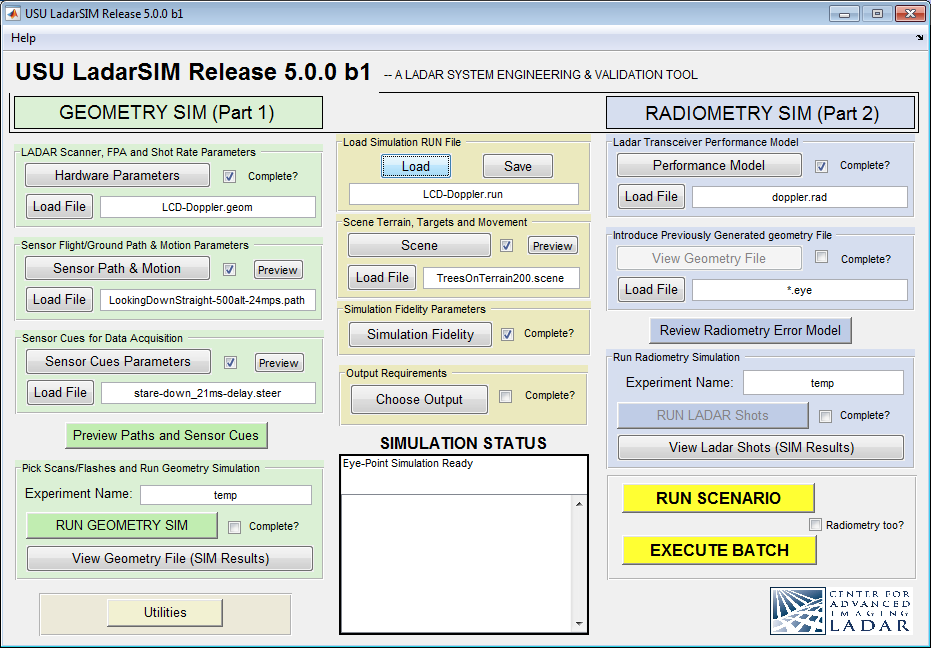
\includegraphics[width=.8\columnwidth]{figs/LadarSIM}
	\vspace{1em}
	\caption{Main GUI for running LadarSIM.}
	\label{fig:LadarSIM}
\end{figure}
    \chapter{Frequency Modulated Continuous Wave Detection}

\section{FMCW Radar}
\label{sec:FMCWRadar}

The theory behind Frequency Modulated Continuous Wave (FMCW) detection will 
be explored in this section following the development of Brooker\cite{brooker2009}.
Booker's development focuses on FMCW radar, but the same theory applies to 
FMCW lidar by making the appropriate changes in the system hardware. For example, 
the antennae would be replaced with a telescope etc.   

\subsection{Basic Principles}

FMCW detection refers to a radar/lidar 
system in which a continuous wave of known frequency is modulated in amplitude,
transmitted, and the reflected signal is detected. A continuous wave radar in 
which a single microwave oscillator serves as both
the transmitter and local oscillator (LO) is, generally speaking, a homodyne radar.
Frequency modulated continuous waveform (FMCW) radar systems often leverage a 
homodyne architecture.

An FMCW radar uses a continuous wave signal which is modulated in amplitude 
over a range of frequencies creating a linear chirp. This chirped signal is 
radiated to the target and an echo 
returns after time $T_p$, which is the time it takes for the signal to reach the
target and reflected energy to return to the antennae. Figure~\ref{fig:doppShift}
illustrates a chirped signal, shown with a solid line, and the return signal delayed
by $T_p$, shown with a dashed line. In this figure $f_b$ refers to the difference in 
frequency of the two signals at a given time.  

\begin{figure}
	\begin{center}
		\begin{tikzpicture}[every text node part/.style={align=center}]
			\draw[thick,->] (1,1) -- (7,1) node[anchor=north] {Time};
			\draw[thick,->] (1,1) -- (1,5) node[anchor=south] {Freq};
			\draw (1,1) -- (5,5);
			\draw[dashed] (2.5,1) -- (6.5,5);
			\draw[dashed,<->] (4,2.6) -- (4,3.9) node[pos=0.5, anchor = east] {$f_b$};
			\draw[dashed,<->] (1,.8) -- (2.5,.8) node[pos=0.5, anchor = north] {$T_p$};
			\draw[dashed,<->] (1,0) -- (5,0) node[pos=0.5, anchor = north] {$T_b$};
		\end{tikzpicture}
		\caption{Transmit and Receive Doppler Shift}
		\label{fig:doppShift}
	\end{center}
\end{figure}

It is clear that the distance to the target can be calculated with $T_p$. In an FMCW system
$T_p$ is determined by measuring the beat frequency $f_b$. To do this a portion of the signal
produced by the LO is mixed with the returned echo producing $f_b$. A signal chirped in frequency
can be expressed as

\begin{equation}
\label{eq:chirpSig}
v_{fm}(t)=A_c cos[\omega_ct+\frac{A_b}{2} t^2].
\end{equation}

Where $A_b$ is a constant of proportionality between the change in frequency over the chirp or chirp slope, $\omega_b$,
and the chirp time; such that $\omega_b=A_bt$. The mixture of the transmitted and received signals can be 
expressed as

\begin{equation}
\label{eq:mixSig}
v_{fm}(t-T_p)v_{fm}(t)=A_c^2 cos[\omega_c t +\frac{A_b}{2}t^2]cos[\omega_c(t-T_p)+\frac{A_b}{2} (t-T_p)^2].
\end{equation}

This simplifies to 

\begin{equation}
\label{eq:mixSigOut}
v_{out}(t)=A_c^2 (cos[(2\omega_c-A_bT_p)t+A_bt^2+(\frac{A_b}{2}T_p^2-\omega_cT_p)]+cos[A_bT_pt+(\omega_cT_p-\frac{A_b}{2}T_p^2)]).
\end{equation}

It is desirable to isolate the second term in Eq~\ref{eq:mixSigOut} because it is the the beat signal. 
The first cosine term is an FM chirp at about twice the carrier frequency and is in most cases 
conveniently filtered out because it is above the cutoff frequency of the receiver components.
To obtain the $f_b$ from the beat signal the phase term is differentiated with time, 

\begin{equation}
\label{eq:phaseDiff}
f_b=\frac{1}{2\pi}\frac{d}{dt}[A_bT_bt+(\omega_cT_p-\frac{A_b}{2}T_p^2)],
\end{equation}

resulting with

\begin{equation}
\label{eq:fb}
f_b=(\frac{A_b}{2\pi})T_p.
\end{equation}

\subsection{FMCW Detection}
As discussed above, the most common way to obtain the beat frequency, $f_b$, is to 
take the product of the transmitted chirp signal and the received signal and filter 
to isolate the constant frequency beat. The Fast Fourier Transform (FFT) is the most
common method of spectral analysis employed in FMCW radar to measure $f_b$. 

Given a chirp duration, $T_b$(s), and assuming that $T_b$$\gg$$T_p$, the maximum resolution
of the beat frequency is 2/$T_b$(Hz). Figure \ref*{fig:doppShift} shows a chirp which meets 
that criterion. The resolution bandwidth of a signal, $\delta$$f_b$, is commonly defined 
between its 3 dB points. For the truncated chirp case  $\delta$$f_b$ coincides with a
region of width 1/$T_b$ centered on $f_b$, as shown in figure \ref{fig:trunkSpect}. 

\begin{figure}
	\begin{center}
		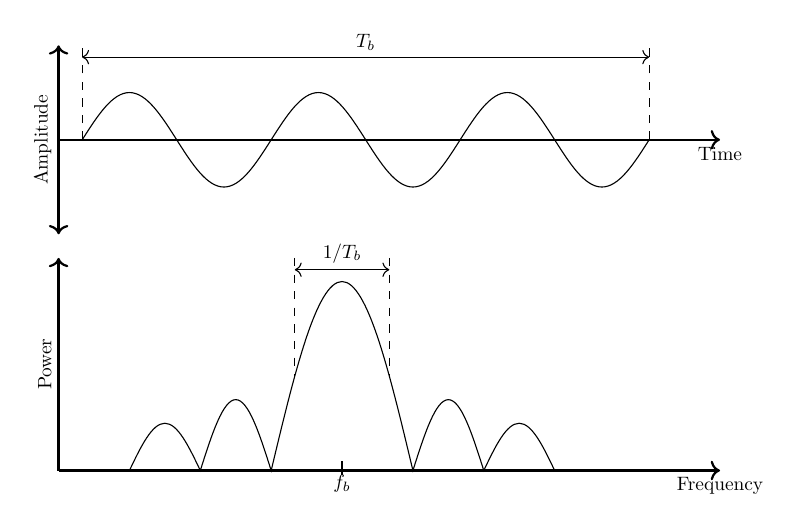
\begin{tikzpicture}[scale = .6,every text node part/.style={align=center}]
		\draw[thick,->] (1,8) -- (15,8) node[anchor=north,scale=0.7] {Time};
		\draw[thick,<->] (1,6) -- (1,10) node[pos = 0.5,above,scale=0.7,rotate=90] {Amplitude};
		\draw[thick,->] (1,1) -- (15,1) node[anchor=north,scale=0.7] {Frequency};
		\draw[thick,->] (1,1) -- (1,5.5) node[pos = 0.5,above,scale=0.7,rotate=90] {Power};
		\draw (2.5,1) sin (3.25,2) cos (4,1) sin (4.75,2.5) cos (5.5,1)  sin (7,5)  cos (8.5,1)
		sin (9.25,2.5) cos (10,1) sin (10.75,2) cos (11.5,1);  
		\draw (1.5,8) sin (2.5,9) cos (3.5,8) sin (4.5,7) cos (5.5,8) sin (6.5,9) cos (7.5,8)
		sin (8.5,7) cos (9.5,8) sin (10.5,9) cos (11.5,8) sin (12.5,7) cos (13.5,8);
		\draw[<->] (1.5,9.75) -- (13.5,9.75) node[pos = 0.5,anchor = south,scale=0.7] {$T_b$};
		\draw[dashed] (1.5,8) -- (1.5,10);
		\draw[dashed] (13.5,8) -- (13.5,10);
		\draw[<->] (6,5.25) -- (8,5.25) node[pos = 0.5,anchor = south,scale=0.7] {1/$T_b$};
		\draw[dashed] (6,5.5) -- (6,3);
		\draw[dashed] (8,5.5) -- (8,3);
		\draw (7,1.2) -- (7,.9) node[pos=0.5,below,scale=0.7] {$f_b$};
		\end{tikzpicture}
		\caption{Spectrum of the truncated sinusoidal signal output by an FMCW radar.}
		\label{fig:trunkSpect}
	\end{center}
\end{figure}

The chirp bandwidth is the total change in frequency for the chirp, $\Delta$$f$. Clearly
the slope of the chirp is the chirp bandwidth divided by the chirp time, $\Delta$$f$/$T_b$.
Eq \ref{eq:fb} can then be restated

\begin{equation}
	\label{eq:fb_alt}
	f_b=(\frac{A_b}{2\pi})T_p=\frac{\Delta f}{T_b}T_p.
\end{equation}

Intuitively $T_p$ is the round trip time from the antennae to the target and back

\begin{equation}
	\label{eq:roundTrip}
	T_p=2\frac{2R}{c},
\end{equation}

where c is the speed of light. The classical FMCW formula is obtained by substituting 
into eq \ref{eq:fb_alt}:

\begin{equation}
	\label{eq:classicFMCW}
	f_b=\frac{\Delta f}{T_b}\frac{2R}{c},
\end{equation}

relating the beat frequency to the range. Solving for range yields

\begin{equation}
\label{eq:FMCWrange}
R=\frac{T_bc}{2\Delta f}f_b.
\end{equation}

Eq \ref{eq:FMCWrange} relates range to beat frequency. The same equation can be used
to related range resolution $\delta$$f$ and chirp bandwidth:

\begin{equation}
	\label{eq:FMCWres}
	\delta R=\frac{T_bc}{2\Delta f}\delta f=\frac{c}{2\Delta f}.
\end{equation}

Where the frequency resolution $delta$$f$ is approximately equal to 1/$T_b$. 

\subsection{Doppler Effect in FMCW}
So far the development in this section has assumed a stationary radar and target. The 
case where the radar, the target, or both are moving will now be examined. The Doppler 
effect describes the change in observed and transmitted frequencies when the distance 
between the two is changing. The relationship between the transmitted frequency, $f_c$, 
and the received frequency, $f_r$ can be expressed

\begin{equation}
	\label{eq:dop1}
	f_r=\frac{c+v_t}{c+v_s}f_c.
\end{equation}

Where $v_t$ is the velocity of the target and $v_s$ is the velocity of the source. From
eq \ref{eq:dop1} it is simple to obtain an equation for the change in frequency, $\Delta$f
in relation to the difference in velocity of the source and target, $\Delta$$v$:

 \begin{equation}
 \label{eq:dop2}
 \Delta f=\frac{\Delta v}{c}f_s.
 \end{equation}
 
 For the following development the radial velocity, $v_r$(m/s), will represent the velocity 
 term causing the Doppler effect. Modifying eq \ref{eq:chirpSig} to incorporate the Doppler 
 shift of the echo signal yields:
 
 \begin{equation}
	 \label{eq:chirpSigDop}
	 v_{fm}(t-T_p)=A_c cos[\omega_c(t-T_p)+\frac{A_b}{2} (t-T_p)^2-\frac{2v_r}{c}\omega_c(t-T_p)].
 \end{equation}
  
The new beat frequency then is the same as derived in eqs \ref{eq:fb} and \ref{eq:fb_alt} shifted
by the Doppler frequency, $f_d$:

\begin{equation}
	\label{eq:fbDop}
	f_b=\frac{2v_r}{c}f_c-\frac{A_b}{2\pi}T_p
	  =f_d-\frac{A_b}{2\pi}T_p.
\end{equation}

For a chirp with positive $A_b$, an up-chirp, the beat frequency will be the difference between 
the Doppler frequency $f_d$ and the beat frequency caused by the echo time or range frequency $f_r$. For a down-chirp, a negative
slope, the beat frequency will be the sum of the Doppler frequency and the range frequency. In many radar applications
it can be assumed that the Doppler frequency is lower than the range frequency leading to eqs \ref{eq:fbUp} and \ref{eq:fbDown}.
If $f_d$ > $f_b$, as is frequently the case in Lidar, the roles of $f_d$ and $f_b$ are reversed. 

\begin{equation}
\label{eq:fbUp}
f_{bUp}=f_b - f_d
\end{equation}

\begin{equation}
\label{eq:fbDown}
f_{bDown}=f_b + f_d
\end{equation}

By using a triangle waveform the sum and difference frequencies can be obtained to isolated range and velocity measurements. 
Fig \ref{fig:UpDownChirp} illustrates the Doppler effect on an FMCW waveform transmitting a triangle wave pattern.  
Expressions for $f_r$ and $f_d$ can be obtained by averaging and differencing eqs  \ref{eq:fbUp} and \ref{eq:fbDown}:

 \begin{equation}
 \label{eq:fr}
 f_r = \frac{f_{b(up)}+f_{b(down)}}{2},
 \end{equation}

 \begin{equation}
\label{eq:fd}
f_d = \frac{f_{b(up)}-f_{b(down)}{2}.
\end{equation}

The sign of $f_d$ is determined by the direction of motion. If the range is getting smaller $f_d$ will be positive 
and if the range is getting larger $f_d$ will be negative. 

\begin{figure}
	\begin{center}
		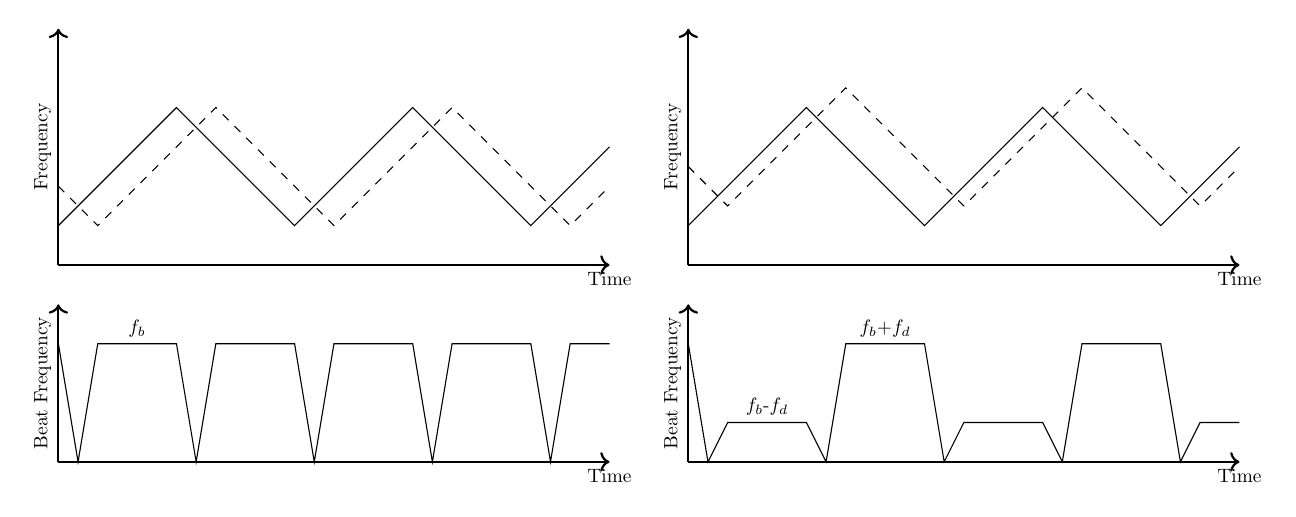
\begin{tikzpicture}[scale = .5,every text node part/.style={align=center}]
		%Left set of graphs
		\draw[thick,->] (1,6) -- (15,6) node[anchor=north,scale=0.7] {Time};
		\draw[thick,->] (1,6) -- (1,12) node[pos = 0.5,above,scale=0.7,rotate=90] {Frequency};
		\draw[thick,->] (1,1) -- (15,1) node[anchor=north,scale=0.7] {Time};
		\draw[thick,->] (1,1) -- (1,5) node[pos = 0.5,above,scale=0.7,rotate=90] {Beat Frequency};
		%transmit
		\draw (1,7) -- (4,10) -- (7,7) -- (10,10) -- (13,7) -- (15,9);
		\draw[dashed] (1,8) -- (2,7) -- (5,10) -- (8,7) -- (11,10) -- (14,7) -- (15,8);
		
		%beat
		\draw (1,4) -- (1.5,1) -- (2,4) -- (4,4) -- (4.5,1) -- (5,4) -- (7,4) -- (7.5,1) -- (8,4)
			  -- (10,4) -- (10.5,1) -- (11,4) -- (13,4) -- (13.5,1) -- (14,4) -- (15,4);
		\draw (2,4) -- (4,4) node[pos = 0.5,above,scale=0.7] {$f_b$};
		
		
		%Right set of graphs
		\draw[thick,->] (17,6) -- (31,6) node[anchor=north,scale=0.7] {Time};
		\draw[thick,->] (17,6) -- (17,12) node[pos = 0.5,above,scale=0.7,rotate=90] {Frequency};
		\draw[thick,->] (17,1) -- (31,1) node[anchor=north,scale=0.7] {Time};
		\draw[thick,->] (17,1) -- (17,5) node[pos = 0.5,above,scale=0.7,rotate=90] {Beat Frequency};
		%transmit
		\draw (17,7) -- (20,10) -- (23,7) -- (26,10) -- (29,7) -- (31,9);
		\draw[dashed] (17,8.5) -- (18,7.5) -- (21,10.5) -- (24,7.5) -- (27,10.5) -- (30,7.5) -- (31,8.5);
		
		%beat
		\draw (17,4) -- (17.5,1) -- (18,2) -- (20,2) -- (20.5,1) -- (21,4) -- (23,4) -- (23.5,1) -- (24,2)
		-- (26,2) -- (26.5,1) -- (27,4) -- (29,4) -- (29.5,1) -- (30,2) -- (31,2);
		
		\draw (18,2) -- (20,2) node[pos = 0.5,above,scale=0.7] {$f_b$-$f_d$};
		\draw (21,4) -- (23,4) node[pos = 0.5,above,scale=0.7] {$f_b$+$f_d$};
		
		\end{tikzpicture}
		\caption{Doppler Effect on FMCW radar.}
		\label{fig:UpDownChirp}
	\end{center}
\end{figure}



\section{FMCW Lidar}
\label{sec:FMCWLidar}

The above section explored the basic functionality of FMCW radar. These basic concepts can be used
to develop an FMCW lidar system. This change leads to very few alterations to the equations in section
\ref{sec:FMCWRadar}, most notably that in many lidar systems $f_d$ will be greater than $f_b$. 
In this section a number of detection architectures for FMCW lidar will be examined. Adany et al. provide
and analysis of direct detection, heterodyne detection, as well as their proposed simplified homodyne 
detection \cite{adany09,adany2007simplified} which will serve as the primary source of information in this section. 

\subsection{Direct Detection Architecture}
In an FMCW direct detection scheme, the signal from the modulation waveform generator is split. Part of the signal
is used to modulate the amplitude of the laser, which is then amplified and sent to the telescope. The 
returning light is captured through the same telescope and converted into an electrical signal via a
photo detector. The other part of the modulation signal is then mixed with the electrical signal from the
detected returning light to perform de-chirping. An FFT is then taken on the de-chirped signal to find 
the beat frequency and the range information. The returning signal is weak so the signal to noise ratio (SNR)
at the output of the photodiode is primarily limited by thermal noise. Considering only thermal noise leads
to the following expression for the maximum SNR:

\begin{equation}
\label{eq:directSNR}
SNR_{dir}\approx\frac{2\Re^2P_{sig}^2}{\frac{4kTB_e}{R_L}}. 
\end{equation}
  
Where $\Re$ is the photodiode responsivity, $P_{sig}$ is the optical power of the received sigal, $k$ is Planck's
constant, $T$ is the absolute temperature, $B_e$ is the electrical bandwidth, and $R_L$ is the load resistance.
Analysis of eq \ref{eq:directSNR} shows that for every dB reduction in the return signal power the SNR is reduced
by 2 dB. This disadvantage leads to very quick degradation of the performance of a lidar system using direct detection
as range increases. 

\begin{figure}[H]
	\centering
	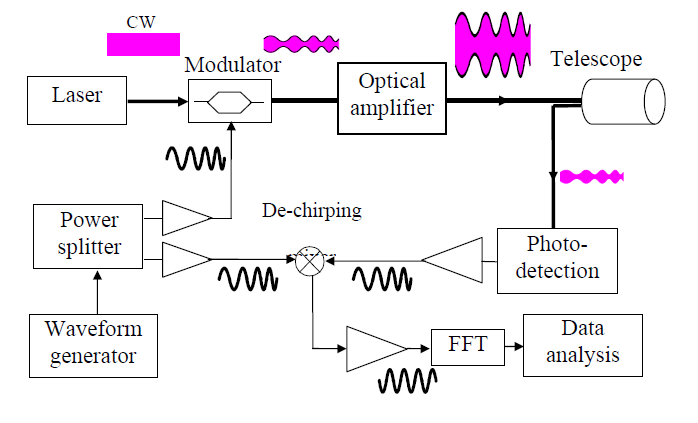
\includegraphics[width=0.8\columnwidth]{figs/direct}
	\vspace{1em}
	\caption{Direct detection architecture}
	\label{fig:directBlock}
\end{figure}

\subsection{Coherent Heterodyne Detection Architecture}
In coherent heterodyne detection the laser is split into two signals. One of these signals is modulated by the 
chirp waveform sent through an optical amplifier and out of the telescope. The other part of the the laser beam 
is used as the optical local oscillator. This LO signal is then shifted by an acousto-optic modulator to serve as
the intermediate frequency (IF) for coherent heterodyne detection. The IF is optically mixed with the returning 
signal from the telescope, the output of the optical mixer is fed into a balanced photodiode. The photodiode 
rejects the direct detection component. The output of the photodiode is filtered to isolate the heterdyne IF 
signal which is detected by an envelope detector. The IF signal is then mixed with the modulation waveform 
for dechirping. An FFT is then performed on the dechirped signal to recover the beat frequency.  

Optically mixing the returned signal with the LO helps mitigate the thermal noise in the photodiode. But because
the strong optical LO, the SNR is limited by the shot noise. The theoretical best SNR for a coherent heterodyne 
lidar is

\begin{equation}
\label{eq:heteroSNR}
SNR_{het}\approx\frac{\Re P_{sig}}{2qB_e}. 
\end{equation}

In this equation q is the electron charge. In coherent heterodyne detection the SNR is linearly proportional to 
the optical power, making it more suitable for low power operation. The most significant disadvantage of coherent
heterodyne detection is its complexity. The IF must be set much higher than the baseband, often in the GHz. This 
necessitates high speed optical detection and radio frequency (RF) processing circuitry. The IF envelope detection
process mixes the signal with RF noise which can further limit the SNR. Because of this the theoretical SNR defined
in eq \ref{eq:heteroSNR} has not been obtained in a coherent heterodyne implementation \cite{1319mmPerf}.  

\begin{figure}[H]
	\centering
	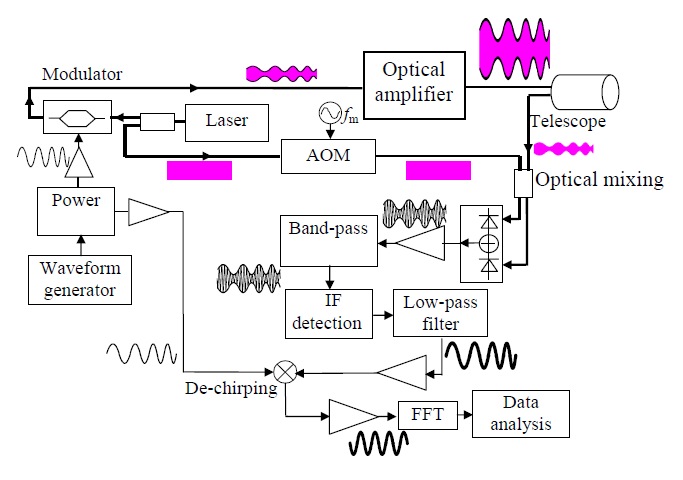
\includegraphics[width=0.8\columnwidth]{figs/heterodyne}
	\vspace{1em}
	\caption{Coherent heterodyne detection architecture}
	\label{fig:heterodyneBlock}
\end{figure}


\subsection{Homodyne Self-Chirped Detection Architecture}
The homodyne self-chirped architecture was developed to maintain the receiver sensitivity obtained from coherent
heterodyne detection while minimizing complexity. In this simplified homodyne detection scheme the laser is 
modulated by the chirp waveform then split in two. One part of the modulated laser is amplified and sent out the
telescope, the other is used as the LO. The returned laser signal is mixed with the LO via a 2x2 optical coupler
the output of which is fed into a balanced photodetector. Because the LO is modulated with the same waveform as 
the transmitted laser, the optical mixing performs both optical detection and RF de-chirping. This reduces the 
amount of RF noise which is introduced to the detection signal. Performing an FFT on the output of the photodetector
yields the beat frequency. 

The simplification of the signal path in the homodyne self-chirped architecture results in a practical SNR closer
to the theoretical SNR in eq \ref{eq:heteroSNR} than the practical SNR of the coherent heterodyne architecture. 

\begin{figure}[H]
	\centering
	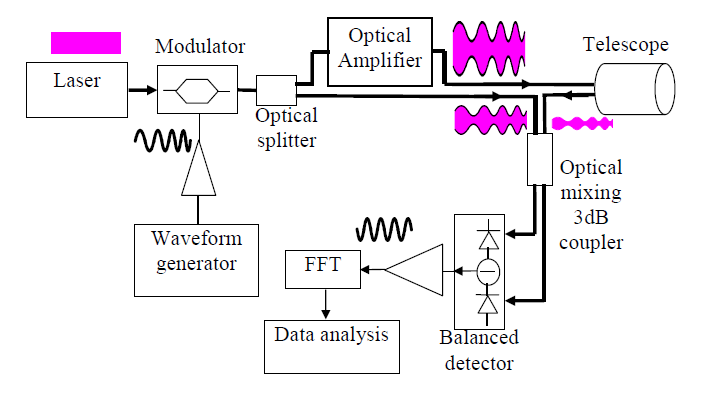
\includegraphics[width=0.8\columnwidth]{figs/simpleHomodyne}
	\vspace{1em}
	\caption{Homodyne self-chirped detection architecture}
	\label{fig:homodyneBlock}
\end{figure}

\subsection{FMCW Lidar Detection}
The two main differences between FMCW lidar and radar are the modulation frequencies and the wavelength of the 
radiation. 






    
    % Endmatter
    % For BibTeX references: specify a .bib file and a style.
    % The style used here is for IEEE transactions formatting:
    \bibliographystyle{IEEEtran}
    \bibliography{myBib}
    % The style used here is for AIAA formatting:
%    \references{IEEEabrv,sample}{aiaa}
    
%    %
%  Example Appendix pages.
%  Modified to use new usu-thesis-mk2 appendix facilities.
%
%  Time-stamp: "[appendix.tex] last modified by Scott Budge (scott) on 2011-08-08 (Monday, 8 August 2011) at 15:46:06 on goga"
%
%  Info: $Id$   USU
%  Revision: $Rev$
% $LastChangedDate$
% $LastChangedBy$
%
%
% For a single appendix, use \makeappendix, and place the 
% body of the appendix after it

%\makeappendix

% < single appendix body here >

% For multiple appendices, use \makeappendices, and create each appendix
% using \appendix{}
% For sub-appendices use \appendixsection{} and \appendixsubsection{}

\makeappendices
\appendix{List of Edge Vectors}
\label{chap:appendix}


\appendixsection{Definition of an Edge Vector}
\label{sec:edge-def}

Before we list the table of edge vectors, we need to describe what an
edge vector is.  In this section we will describe in detail the theory
that results in the edge vectors.  The first set of edge vectors is
given in Table~\ref{table1}.

\begin{table}[!t]
% increase table row spacing, adjust to taste
  \renewcommand{\arraystretch}{1.3}

  \caption{List of edge vectors for a codebook with b=8 and d=3, for a
    $4 \times 4$ vector size.}
  \label{table1}

  \centering
  \begin{tabular}{|c|c|} \hline
    Level & Edge Vectors \\ \hline

    & (5) \\ 
    L1 & (6) \\
    & (7) \\ \hline

    & (3,1)\\
    & (3,2)\\
    & (3,5)\\
    & (4,0)\\
    L2 & (4,2)\\
    & (4,3)\\
    & (4,4)\\
    & (4,5)\\
    & (4,6) \\ \hline

    & (3,4,1)\\
    & (3,4,2)\\
    & (3,7,0)\\
    & (3,7,2)\\
    & (3,7,4)\\
    L3 & (4,1,0)\\
    & (4,1,1)\\
    & (4,1,2)\\
    & (4,1,3)\\
    & (4,1,4)\\
    & (4,1,5)\\
    & (4,1,6) \\ \hline

  \end{tabular}

\end{table}


\appendixsection{Next Codebook Size Description}
\label{sec:next-size}

In this section we do the next size codebook.  This is different from
the previous case in that the codebook size is different.  The next
set of edge vectors is given in Table \ref{table2}.

\appendixsection{Final Set of  Codebook Size Descriptions}
\label{sec:final-size}

The following three tables contain the data for codebook sizes that
are different than the previous sizes.  We note that the differences
in the tables are due to the differences in the sizes of the codebook
edge vectors.  Note the values given in Table \ref{table3} --
Table \ref{table5}.


\begin{table}[!t]
  \renewcommand{\arraystretch}{1.3}
  \centering

  \caption{List of edge vectors for a codebook with b=4 and d=3, for a
    $4 \times 4$ vector size.}
  \label{table2}

  \begin{tabular}{|c|c|} \hline
    Level & Edge Vectors \\ \hline

    & (1)\\
    L1 & (2)\\
    & (3) \\ \hline

    L2 & (0,3) \\ \hline

    & (0,2,0)\\
    L3 & (0,2,2)\\
    & (0,2,3) \\ \hline

  \end{tabular}

\end{table}

\begin{table}[!t]
  \renewcommand{\arraystretch}{1.3}
  \centering

  \caption{List of edge vectors for a codebook with b=16 and d=3, for
    a $4 \times 4$ vector size.}
  \label{table3}

  \begin{tabular}{|c|c|} \hline
    Level & Edge Vectors \\ \hline

    & (11)\\
    & (12)\\
    L1 & (13)\\
    & (14)\\
    & (15) \\ \hline

    & (7,0)\\
    & (7,1)\\
    & (7,2)\\
    & (7,6)\\
    L2 & (8,4)\\
    & (8,5)\\
    & (8,6)\\
    & (9,6)\\
    & (9,14)\\
    & (10,1) \\ \hline

    & (4,6,14)\\
    & (5,6,6)\\
    & (6,14,0)\\
    & (6,14,3)\\
    L3 & (6,14,4)\\
    & (6,14,5)\\
    & (7,7,0)\\
    & (7,14,7)\\
    & (9,5,3)\\
    & (9,5,10)\\
    & (9,5,11) \\ \hline

  \end{tabular}

\end{table}

\begin{table}[!t]
  \renewcommand{\arraystretch}{1.3}
  \centering

  \caption{ List of edge vectors for a codebook with b=16 and d=3, for
    a $2 \times 2$ vector size.}
  \label{table4}

  \begin{tabular}{|c|c|} \hline
    Level & Edge Vectors \\ \hline

    & (9)\\
    & (10)\\
    L1 & (11)\\
    & (12)\\
    & (13) \\ \hline

    L2 & (6,0)\\
    & (6,3) \\ \hline

    & (2,2,8)\\
    & (6,5,1)\\
    & (6,5,4)\\
    & (6,5,6)\\
    & (6,5,7)\\
    & (6,5,8)\\
    L3 & (6,5,15)\\
    & (7,0,14)\\
    & (8,0,1)\\
    & (8,15,3)\\
    & (8,15,4)\\
    & (8,15,10) \\ \hline

  \end{tabular}

\end{table}

\begin{table}[!t]
  \renewcommand{\arraystretch}{1.3}
  \centering

  \caption{ List of edge vectors for a codebook with b=16 and d=3, for
    a $6 \times 6$ vector size.}
  \label{table5}

  \begin{tabular}{|c|c|} \hline
    Level & Edge Vectors \\ \hline

    & (6)\\
    & (7)\\
    & (8)\\
    & (9)\\
    L1 & (10)\\
    & (11)\\
    & (12)\\
    & (13)\\
    & (14)\\
    & (15) \\ \hline

    & (2,8)\\
    & (2,13)\\
    & (4,1)\\
    & (4,6)\\
    L2 & (4,7)\\
    & (4,8)\\
    & (4,10)\\
    & (4,11)\\
    & (4,13)\\
    & (4,15) \\ \hline

    & (1,7,0)\\
    & (1,7,1)\\
    & (1,7,2)\\
    L3 & (1,7,3)\\
    & (1,7,4)\\
    & (1,7,6)\\
    & (1,7,9)\\
    & (1,7,12) \\ \hline

  \end{tabular}

\end{table}

\appendix{Another Example Appendix}


\appendixsection{Background}
\label{sec:back}


Some random appended text for this section of the appendix....


\appendixsection{Meat of the Appendix}
\label{sec:meat}

Here we have the data that is so important to be included in this
appendix.

%    %
% This is an example of a vita page.  
% Format is not tightly specified. This example comes from Lili Ma.
%
%  Time-stamp: "[vita.tex] last modified by Scott Budge (scott) on 2012-07-16 (Monday, 16 July 2012) at 11:18:06 on goga"
%
%  Info: $Id$   USU
%  Revision: $Rev$
% $LastChangedDate$
% $LastChangedBy$
%

\begin{vita}

\begin{center}
{\Large \bf John Q. Engineer}\\
\end{center}

\section*{Published Journal Articles}
    \begin{itemize}
    \item Rational Radial Distortion Models of Camera Lenses with Analytical Solution for Distortion Correction, Lili
    Ma, YangQuan Chen, and Kevin L. Moore, {\it International Journal of Information Acquisition}, {\it Accepted}.

    \item A Small Mobile Robot for Security and Inspection Operations, N.S. Flann, K. L. Moore, and Lili Ma, {\it Control Engineering Practice}, vol. 10, pp. 1265-1270,
    2002.
    \end{itemize}

\section*{Published Conference Papers}
    \begin{itemize}
    \item Range Identification for Perspective Dynamic Systems Using
      Linear Approximation, Lili Ma, YangQuan Chen, and Kevin
      L. Moore, in {\it Proc. IEEE Int. Conf. on Robotics and
        Automation (ICRA)},
    2004.
  \item Range Identification for Perspective Dynamic System with
    Single Homogeneous Observation, Lili Ma, YangQuan Chen, and Kevin
    L. Moore, in {\it Proc. IEEE Int. Conf. on Robotics and Automation (ICRA)},
    2004.
  \item Blind Detection and Compensation of Camera Lens Geometrical
    Distortions, Lili Ma and YangQuan Chen, {\it SIAM Imaging
      Science}, 2004.
  \item Flexible Camera Calibration Using a New Analytical Radial
    Undistortion Formula with Application to Mobile Robot
    Localization, Lili Ma, YangQuan Chen, and Kevin L. Moore, in {\it
      Proc. Int. Symposium on Intelligent Control (ISIC)}, 2003.
  \item Sonar and Laser Based HIMM Map Building for Collision
    Avoidance for Mobile Robots, Lili Ma and Kevin L. Moore, in {\it
      Proc. International Symposium on Intelligent Control (ISIC)},
    2003.
  \item Wireless Visual Servoing for ODIS - An Under Car Inspection
    Mobile Robot, Lili Ma, Matthew Berkemeier, YangQuan Chen, Morgan
    Davidson, Vikas Bahl, and Kevin L. Moore, in {\it Proc. IFAC World
      Congress}, Spain, July, 2002.
  \item Visual Servoing of an Omni-Directional Mobile Robot for
    Alignment with Parking Lot Lines, Matthew Berkemeier, Morgan
    Davidson, Vikas Bahl, YangQuan Chen, and Lili Ma, in {\it Proc.
      IEEE Int.  Conf. on Robotics and Automation (ICRA)}, May 2002.
  \item Some Sensing and Perception Techniques for an Omnidirectional
    Ground Vehicle with a Laser Scanner, Zhen Song, YangQuan Chen,
    Lili Ma, and You Chung Chung, in {\it Proc. IEEE Int. Symposium on
      Intelligent Control (ISIC)}, October 2002.
  \item A Small Mobile Robot For Security and Inspection Operations,
    Flann NS, Moore KL, and Ma L, in {\it Proc. IFAC Conference on Telematics
      Applications in Automation and Robotics}, July 2001.
    \end{itemize}

\end{vita}

    %}}}
\end{document}
